% http://www.idsc.ethz.ch/education/theses-semester-projects.html
% IDSC LaTeX Thesis Template
% 
% Author(s):	Eric Müller
% 				Institute for Dynamic Systems and Control
% 				Swiss Federal Institute of Technology (ETH) Zurich
% 
% Created:		2004/04/02  (Eric Mueller)
% 
% Notes: Has been tested on Windows 7 + MikTeX + TeXnicCenter
%
% Revisions: 	2009/05/29  (Soren Ebbesen)
% 				    2011/03/22	(Soren Ebbesen)
%             2013/03/08	(Soren Ebbesen)
%             2014/03/13	(Soren Ebbesen)
% ______________________________________________________________________________
\documentclass[12pt,oneside,a4paper,fleqn]{article}
\usepackage{siunitx}
%\usepackage[utf8]{inputenc}
\usepackage[onehalfspacing]{setspace}
%\usepackage{lineno}\linenumbers

% CHANGE HERE FOR GERMAN (german) OR MASTER THESIS (mt)!!!!!

\usepackage[english,bt]{ethidsc} % Special IDSC styles and commands      	
								 % {german}/english: language of headings, etc.
								 % {st}/bt/mt: {semester}/bachelor/master thes
\addbibresource{references.bib}
\usepackage{calligra}
\usepackage{mathtools}
\usepackage{amsmath}
\usepackage{float}
\usepackage{siunitx} 
\usepackage{array}
\usepackage{hyperref}
\usepackage{graphicx}
\usepackage{booktabs}
\usepackage{geometry}
\usepackage{subcaption}
\usepackage{amssymb}
\usepackage{microtype}
\usepackage{braket}
\usepackage{cleveref}
\usepackage{wrapfig}

% Page header (don't change)____________________________________________________
\setlength{\parindent}{0em}                 % Disable parindent
\rhead[\nouppercase{\rightmark}]{\thepage}  % Special headings
\lhead[\thepage]{\nouppercase{\leftmark}}   % Special headings
\cfoot{}                                    % Special headings


% Title page (please fill in)___________________________________________________
\title{Influence of probabilistic abstention on spatial cooperative games}


\studentA{Alessandro Azzani, Francesco Gargiulo \\ Lea Haas}
%\ethidA{20-000-00}
%\semesterA{6}
%\emailA{someone@student.ethz.ch}

\studentB{Nicol\`{o} Montalti}
%\ethidB{12-345-678}
%\semesterB{9}
%\emailB{second@student.ethz.ch}

%\supervision{Prof. Dr. Superviser}
\date{\today}

%\identification{IDSC-XX-YY-ZZ} 		% Project identifier

%\infopage
%\declaration

% Begin document________________________________________________________________
\begin{document}

\maketitle 							% Create title page

\pagenumbering{roman}
\tableofcontents
\newpage
% Preamble______________________________________________________________________

%\pagenumbering{roman} 				% Begin roman page numbering (i,ii,...)

%\input{chapters/preamble} %Abstract etc.

% Chapters______________________________________________________________________

\pagestyle{fancy}               	% Fancy headings			
\setlength{\parindent}{20pt}

% We start writing from here -----------------------------------------------------
\addcontentsline{toc}{section}{Individual contributions}
\section*{Individual contributions}
\label{chap:indv}

Lea Haas has written the Theoretical background section and the introduction. She focused on the theory behind the project and the interpretation of the games we were playing. Nicolò Montalti and Alessandro Azzani have developed the code, generated the results and written the Implementation section. Francesco Gargiulo has helped writing the code, interpreted the results and written the Results and Conclusion sections. Everyone has reviewed the whole report, adding their contribution to other sections. The same division of work was applied to the presentation.

\newpage
\addcontentsline{toc}{section}{Introduction}
\section*{Introduction}
\label{chap:intro}
\pagenumbering{arabic}

In the study of games how cooperative behaviour emerges in social dilemmas has always been an intriguing topic. Understanding the factors that promote cooperation among individuals is crucial for comprehending the dynamics of human interaction and decision-making.

In this report, we look at spatial evolutionary games and how probabilistic abstention can encourage cooperation. Our study focuses on four distinctive games: the Prisoner's Dilemma, Stag Hunt, Harmony and Snowdrift Game. Each of these games captures different aspects of social dilemmas. We use a spatial setup to allow for localized interactions and the emergence of spatial patterns. This framework provides a more realistic representation of social scenarios. By using the dynamics of evolutionary game theory, we simulate how the player's strategies evolve over time. We examine especially the influence of abstention. This has been done before for the prisoner's dilemma \cite{cardinot2018}. \\Two questions are important for this analysis:

\begin{itemize}
    \item Can abstention promote cooperation in games other than the prisoners dilemma?
    \item What is the correlation between having a certain abstention probability and having the strategy cooperation/defection?
    \item In games where cooperation is already the dominant strategy, can abstention promote defection?
\end{itemize}

To lay a solid foundation for our analysis, we first start with a theory section that also provides backgrounds on the fields of interest. We then go on to an explanation of how the code is implemented. After that, we discuss our results and draw conclusions.

\section{Theoretical background}
In this section, we want to elaborate on the theoretical background of the project and the connection to Game Theory. We also give an introduction to the relevant fields of study, namely evolutionary game theory and spacial games.

\subsection{Games}
We focus on a very simple model of an interaction between two players. Both of the two players have to make a decision, their choice is called strategy. Depending on their choice and the choice of the other player, they get a payoff. Here, each player has to choose between two different strategies: cooperation (C) or defection (D). This leads to a 2x2 payoff matrix, which is symmetric in all games we consider. Therefore, it is enough to look at the payoff of one player, as shown in \Cref{tab:payoff_matrix}.

\begin{table}[H]
    \centering
    \begin{tabular}{c|c|c}
                               & If the co-player plays C & If the co-player plays D \\
        \hline
        If I play C, I receive & Reward $R$               & Sucker’s payoff $S$      \\
        \hline
        If I play D, I receive & Temptation $T$           & Punishment $P$           \\
    \end{tabular}
    \caption{Payoff matrix for symmetric 2x2 games, taken from \cite{nowak_sigmund_2000}}
    \label{tab:payoff_matrix}
\end{table}

Assuming that $T$ and $R$ are always bigger than $S$ and $P$, there are four different games, which we will look at in the following.

\subsubsection{Prisoner's dilemma (PD)}
The prisoner's dilemma is characterized by $T > R > P > S$, together with $2R > T+S$. It is one of the most famous games in game theory and has been widely examined. It describes a situation where cooperation could lead to high total payoffs but from the point of view of a single player defection is always the better option. Therefore defection is the dominant strategy. This depicts the well-known dilemma between a common good and selfish interests. There can be found different applications as well as in human societies as in the animal world. For example vampire bats that feed each other, like described in Sigmund \emph{et al.} \cite{sigmund1999evolutionary}.

\subsubsection{Snowdrift Game (SD)}
The snowdrift game is also called chicken game or hawk-dove game. Like in the prisoner's dilemma, $T > R$. This means that also here, cooperation is threatened by the temptation $T$. The difference is that the sucker's payoff is bigger than the punishment, $S > P$. So if it is known that one player does not cooperate, it is favourable for the other player to cooperate. Therefore there is no dominant strategy (one that is always favourable): because of the low $P$, you would assume that both players always choose to cooperate. But if you suspect the other player to cooperate, defection is the better option. A common example is a situation where two car drivers are stuck in a snowdrift (\cite{sugden1986economics}, p.132). Cooperation means digging a path through the snow. If the other person refuses to dig, it is still better to dig alone than doing nothing.
%also mention hawk dove like in paper of evolutionary biology?

\subsubsection{Stag Hunt(SH)}
In the stag hunt $R > T > P \geq S$. So here, not the temptation $T$ but rather the punishment $P$ threatens the cooperation. The typical example is two hunters in a forest (\cite{sugden1986economics}, p.202). Alone, they can both hunt for hares. But if they work together, they are able to hunt for deer, which gives them a higher payoff. Also here, there is no dominant strategy. Both cooperating is the best option, but it requires them to trust each other. This game introduces a coordination problem: if one player suspect the other person to defect, it also better for them to defect. So the outcome highly depends on the action of the other player, and it is the best to take the same action as the other player.
%maybe some applications

\subsubsection{Harmony Game (HG)}
The last game has the property $R > T > S > P$ and it's called harmony game. This game is not very commonly used, as cooperation is the dominant strategy. Without having to think and without any twists, both players can choose to cooperate.

\subsection{Repeated Games}
So far, we have always assumed that the games are only being played once. But what is often more interesting is repeated games where the players have a memory. The repeated prisoners dilemma between the same two players has been widely studied. Also here, strategies that maximize the payoff exists. One famous strategy is the so called "tit for tat" strategy, first introduced by Axelrod \cite{axelrod1984evolution} in 1984. It is very simple: in the first round, the player cooperates and then repeats what the other player does.\\
Another approach than repeating the game and trying to find a suitable strategy, is to let the strategies of the players evolve over time with a certain update algorithm. This is what is done in evolutionary game theory.

\subsection{Evolutionary Game theory}
Evolutionary game theory had its breakthrough with a paper by Maynard Smith and Price in 1973 \cite{smith1973logic}. In this paper, they examined how animals behave in conflicts by simulating a game repeatedly. They assigned different strategies to the players and analysed how these strategies would evolve in a population of players. With this, they could explain why escalating fights with serious injuries are rather rare between animals of the same species.
\\ Generally, evolutionary game theory focuses on strategy changes over time. It combines traditional game theory with evolutionary biology: the change in strategy is viewed as the evolution of a certain behaviour. The games are often played by a population of players with different strategies. A method often used is that for each time step the frequency of each strategy in the population is updated, for example following the replicator equations. So compared to the cases before, the player does not rationally decide which strategy to choose, but the strategies are assigned to the players \cite{epstein1998}.
%evoulutionary stable?

\subsection{Spatial games}
Spacial games are another extension to the classical, two player setup. The players are placed on a grid and repetitively play against their neighbours. Spatial games are very often combined with evolutionary game theory. An early example for this can be found in Axelrod \cite{axelrod1984evolution}. He considers the prisoners dilemma. After the players play against their neighbours, they copy the strategy of the neighbour with the highest total payoff. This strategy update mechanism is called imitation and can also be described with the replicator equation. When placing a player that always plays "D" in the middle of players that play "tit for tat", one can observe fractal snowflake patterns, shown in \Cref{fig:axelrod_snowflake}. Emerging patterns are an important aspect of spacial games.

\begin{figure}[h]
    \centering
    \includegraphics[width=0.7\textwidth]{Images/axelrod_snowflake.png}
    \caption{The snowflake pattern after several rounds of the game (generations). The crosses depict players that always defect, while the white players play tit for tat. Image taken from \cite{axelrod1984evolution}}
    \label{fig:axelrod_snowflake}
\end{figure}

An especially interesting question in this field of study is the evolution of cooperative strategies. As cooperation is a very important ingredient for human societies, it can be insightful to study what drives cooperation in the framework of the simple models we look at. Some of these mechanism are given below.

\subsection{Extensions to the model}

\subsubsection{Migration}
In a 2008 paper, Helbing and Yu considered the prisoner’s dilemma on a spatial grid with the dynamics following the replicator equation (imitation) \cite{helbing_migration_2008}. Having this situation, after some time there are just a certain number of cooperators in small clusters left. Surprisingly, when adding the possibility to migrate to a region with higher payoffs, bigger clusters of cooperators can form. This means that the cooperation is promoted by allowing for migration. The cooperators stay in clusters, as this maximizes their payoff and they can be protected from becoming defectors. On the edges of the clusters, defectors are found that take advantage of the cooperators. So like in Axelrods snowflake, spacial patterns emerge.

\subsubsection{Noise}
In a later paper, they also added noise to the model \cite{Helbing_2009_noise}. This means that with a certain probability, the player does not imitate another strategy but instead gets assigned a random strategy. They showed that the noise suppresses cooperation. But when adding migration, the cooperation clusters still form and are stable against the noise.

\subsubsection{Abstention}
Yet another extension to the model is the introduction of probabilistic abstention. This can also promote cooperation in the spacial prisoners dilemma, as shown by Cardint \emph{et al.} \cite{cardinot2018}. Here, in the beginning of a time step, each player has a certain probability to not play the game. This is called the abstention probability. Note that abstention is not treated like a third option, but in a probabilistic way.
\newline
\newline
In this project, we want to follow what has been done previously and further investigate what potentially promotes cooperation. We not only look at the Prisoners dilemma but also at the three other games introduced before. We use imitation as an update mechanism together with abstention and noise and investigate how this changes the strategies of the players.


\section{Implementation}
The game has been implemented in Python, the code is publicly available on GitHub \cite{montalti2023}.
The spatial environment has been implemented as a $50 \times 50$ 2-dimensional grid.
A player is present at every point of the grid.
Every player is characterized by a strategy (collaborate or defect) and by an abstention probability $\alpha \in [0,1]$.
The game is defined by the five parameters $T, R,  P, S, L$ and by a noise factor $\eta \in [0,1]$.
The first five parameters determine the game played: prisoner dilemma (PD), snowdrift (SD), stag hunt (SH) or harmony game (HG).
\subsection{Initialization}
The game is initialized assigning to each player a random strategy, with a $50-50$ probability, and an abstention probability $\alpha$. The latter can be assigned in three different ways:
\begin{itemize}
    \item no abstention: $\alpha = 0$ for all players. The game is reduced to the standard prisoner's dilemma (PD) or another standard game;
    \item optional abstention: $\alpha = 0$ or $1$ with a $50-50$ probability. The game is reduced to the optional prisoner's dilemma (OPD) or the equivalent for other games;
    \item probabilistic abstention: $\alpha \in [0,1]$. The players have a finite probability of abstention, distributed between 0 and 1 with steps of 0.125. In particular, the values that it can assume are
          $\alpha = \{0, 0.125, 0.25 \dots 1 \}$.
          We call this situation prisoner's dilemma with probabilistic abstention (PDPA) or the equivalent for other games.
\end{itemize}
\subsection{Evolution}
At every iteration of the game, each player plays against their four nearest neighbours.
Each player earns an amount equal to the sum of the payoffs of the four games played.
The payoff of a single match between two players is determined by the game played, the strategy of the two players and by their abstention probability.
Each player joins the game with a probability $1-\alpha$.
If both players join the game, the game is played and payoffs are distributed according to the players strategies.
If one of the players abstains, the game is not played, and both players receive a payoff $L$.

After every player has played, the imitation process begins.
The imitation process is influenced by the noise parameter $\eta$.
In particular, each player randomly changes their strategy to the opposite strategy with a probability $\eta$ and imitates rationally their best performing neighbours with a probability $1-\eta$.
If the imitation option is chosen, the player looks at their four nearest neighbours payoffs, and imitates the strategy of the one who performed the best in the last round.
If more players share the same optimal outcome, a random one is chosen.
In addition to imitating the best-performing player's strategy, the abstention probability of the most performing neighbour is imitated as well.
\subsection{Analysis of the results}
The process is iterated for a fixed number of times $t$ (usually $t=200$).
At each iteration, the players play the game and imitate their neighbours' strategies and abstention probabilities.
At the end of the cycle, some statistics are extracted from the final configuration.
Taking inspiration from Cardinot \emph{et al.} \cite{cardinot2018}, we evaluate the mean abstention probability $\alpha$ and the mean effective cooperation frequency $\varepsilon = (1-\alpha)\cdot (1-s)$, where $s = 0$ for a cooperator and $s=1$ for a defector.
In addition to these two quantities, we also analyse the correlation between being a cooperator and having a low abstention frequency $\alpha$.
To do so, when playing the version of the game with probabilistic abstention, we plot the number of cooperators and defectors for each value of $\alpha$ and compare the results.


\section{Results}
\label{sec:results}
We now presents some of the results we found playing different versions of the games. We start by analyzing the prisoner's dilemma, comparing our results to some previous work and presenting an analysis on the correlation between the players' strategies and abstention probabilities. We then turn our attention to different games and perform a similar analysis.
\subsection{Prisoner's dilemma}
\subsubsection{Comparison with the previous work}
First of all, we started by comparing our results with the ones obtained by Cardinot \emph{et al.} \cite{cardinot2018}. In particular, we compared the dependence of the effective cooperation frequency $\varepsilon$ and of the mean abstention probability $\alpha$ on the temptation payoff $T$ in the prisoner's dilemma game.
This comparison is shown in \Cref{fig: comparison of epsilon and alpha}. Comparing the plots, we find that our results are compatible. In both Cardinot's and our study, probabilistic abstention is found to be an efficient way to enhance cooperativity for a large range of values of $T$. For small $T$s, the majority of players eventually decides to join the game, whereas for larger $T$s a considerable fraction of players decides to abstain. It is interesting to notice that for small $T$s, even if eventually no one is abstaining, the cooperation factor $\varepsilon$ is greater. This implies that the possibility to abstain in the initial phases of the game facilitates cooperator to form collaborative clusters. Once the collaborators have met and are close together, they stop abstaining and play the game collaboratively.
\begin{figure}
    \centering
    \subfloat[]{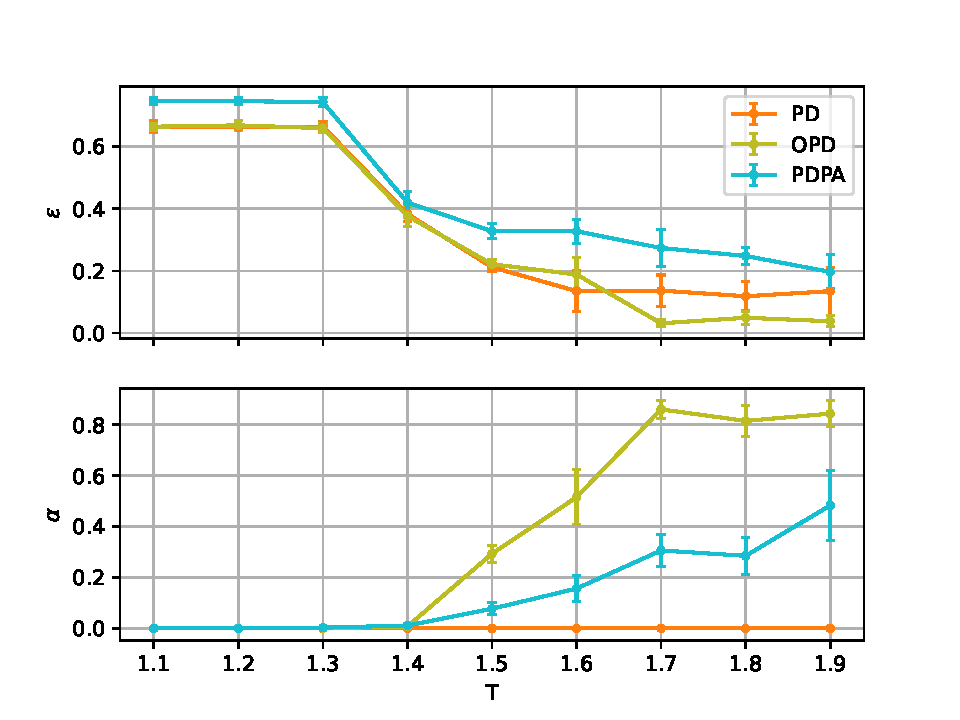
\includegraphics[scale = 0.5]{Images/alpha_eps-20230606-125503.pdf}}
    \subfloat[]{\includegraphics[scale = 0.23]{Images/dependence_of_alpha_and_epsilon_on_T.png}}
    \caption{(a) shows the dependence we obtained for $\alpha$ and $\epsilon$ with respect to $T$ while playing the prisoner's dilemma game, or some variants. The results are obtained plotting the mean and the stanandard deviation of 10 runs with $t=200$ iterations and a noise $\eta = 0.001$. (b) shows to the results of Cardinot \emph{et al.}  \cite{cardinot2018}. Both games have been played with the same parameters $R = 1, S = 0, P = 0, L = 0.4$.}
    \label{fig: comparison of epsilon and alpha}
\end{figure}
While playing the PDPA game, looking at the final configuration of players on the grid, we noticed that for some values of $T$ there was a high correlation between being a defector and having a high abstention probability $\alpha$. Therefore, we decided to better study this correlation comparing the number of cooperators and defectors for each value of alpha.
\subsubsection{Correlation between strategy and abstention}
As we see in \cref{fig:correlation}, most of the cooperators ($> 60 \%$) choose to participate in the game ($\alpha=0$), whereas a minority ($<40\%)$ abstains ($\alpha=1$). The result is explained by the fact that cooperators tend to organise in clusters in order to survive. Inside the cluster, cooperators have the best payoff if they decide to join the game. Nonetheless, some cooperators will play against defectors, so for them the best strategy may be abstaining.
%they want to be surrounded by other cooperators since a defector would have the best outcome if they were to play against a cooperator.
The abstention probabilities for defectors are more spread out. Overall, they have a smaller tendency of joining the game. When defectors are close to each other, they prefer abstaining rather than playing against another defector. This is why we see a higher tendency of defectors that decide to abstain from the game.
\begin{figure}[H]
    \centering
    \includegraphics[width = 0.7 \textwidth]{Images/correlation-20230615-113717.pdf}
    \caption{Correlation between abstention and cooperation. For each value of $\alpha$, the relative number of cooperators is compared to the relative number of defectors. The numbers are normalized dividing by the total number of cooperators/defectors. The marks for cooperators (defectors) are slightly shifted to the left (right) for better readability. Parameters: $T = 1.4, R = 1, S = 0, P = 0.3, L = 0.4$. The results are averaged over 50 repetition of the game, for which we plot the mean and the standard deviation.}
    \label{fig:correlation}
\end{figure}
\subsection{Other games}
After having checked that our results were compatible with the ones derived by Cardinot \emph{et al.}, and having studied the correlation between the strategy and the abstention probability in more detail, we proceeded to analyze different games.
\subsubsection{Snow drift}
We started by looking at the snowdrift game, as shown in \Cref{fig: screenshots of SD OSD SDPA}.
\begin{figure}
    \centering
    \subfloat{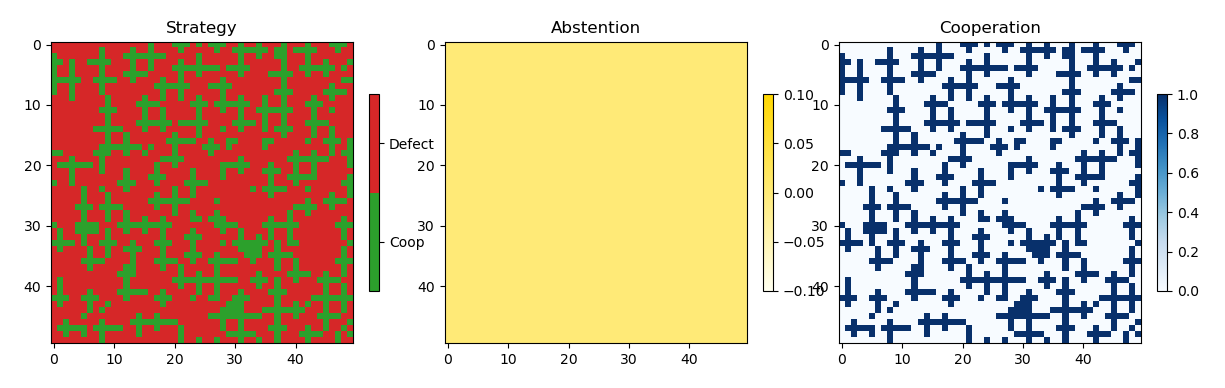
\includegraphics[scale = 0.4]{Images/SD.png}} \\
    \subfloat{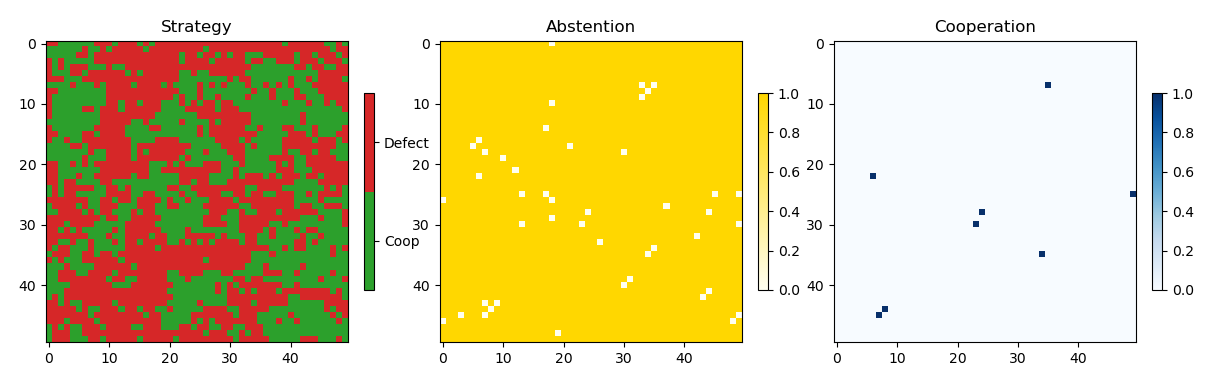
\includegraphics[scale = 0.4]{Images/OSD.png}} \\
    \subfloat{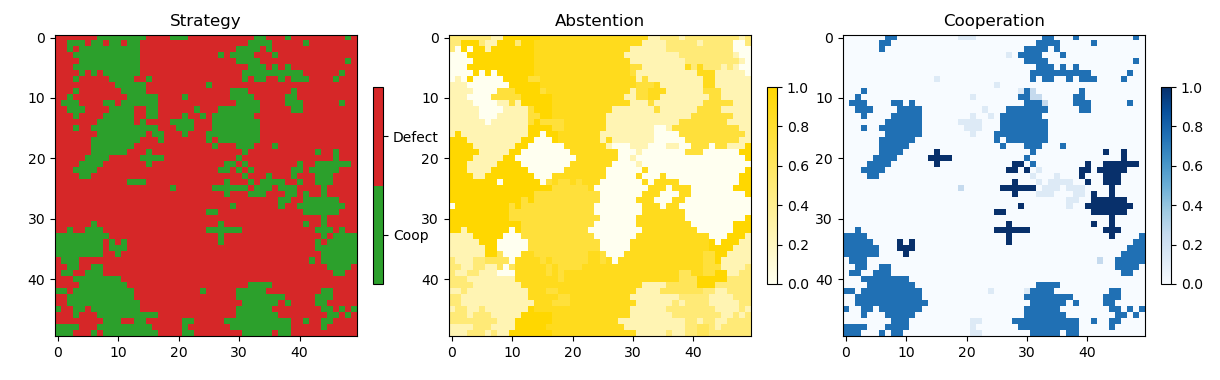
\includegraphics[scale = 0.4]{Images/SDPA.png}} \\
    \caption{Final state of the grid after 200 iterations for three different games (from top to bottom): SD, OSD, SDPA. For each game is shown the final distribution of cooperators and defectors (first column), of the abstention probability $\alpha$ (second column) and of the effective cooperation frequency $\varepsilon$ (last column). All of them have been taken by setting $T = 1.9$. and $\eta = 0.001$}
    \label{fig: screenshots of SD OSD SDPA}
\end{figure}
From the data, it is clear that as soon as we turn on the possibility for the players to abstain, either in a probabilistic or optional way, the clusters of cooperators increase in size.
The most significant difference between the two is that for OPD we notice a bigger tendency of the players to abstain.
On the other hand, when the probability of abstention is randomly generated between $[0,1]$, we observe that some players maintain a values different from 0 and 1.
There also seems to be a correlation between having a low $\alpha$ value and being a cooperator.

\begin{figure}
    \centering
    \includegraphics[scale = 0.7]{Images/alpha_eps_snowdrif.pdf}
    \caption{Dependence of $\alpha$ and $\epsilon$ for the snowdrift game on the parameter $T$. In this case we set $R = 1, S = 0.3, P = 0, L = 0.4, \eta = 0.001$ and $t = 200$. The results are obtained by averaging over 10 different runs.}
    \label{fig: epsilon and alpha snodrift}
\end{figure}

Looking at the average abstention probability $\alpha$ and cooperation factor $\varepsilon$, as shown in \Cref{fig: epsilon and alpha snodrift}, we observe that as long as we keep $T \leq 1.6$, the three games behave in the same way, since no player decides to abstain. All three games are therefore reduced to the standard SD game. The situation is different when we study the game for $T > 1.6$. It can be seen that, while the snowdrift game (SD) gives the same results, the optional snowdrift (OSD) and the snowdrift with probabilistic abstention (SDPA) do not.
Both of them show a non-zero expectation value for the mean abstention probability and a decreasing effective cooperation. In this regime, players stop to be cooperative and prefer  abstaining from the game.
These two effects are more pronounced in the case of the OSD compared to the SDPA.
In fact, since in the OSD the players have either $\alpha = 0$ or $1$ probability to abstain, the system reaches a steady state where all the players decide to not take part in the game.
%Different is the case of the PDPA, where instead some players prefer not to abstain and keep playing, such that the system doesn't actually reach a steady state. 

\begin{figure}
    \centering
    \subfloat[]{\includegraphics[scale = 0.5]{Images/alpha_eps_stag_hunt.pdf}}
    \subfloat[]{\includegraphics[scale = 0.5]{Images/alpha_eps_harmony_game.pdf}}{}
    \caption{(a) show the dependence of $\epsilon$ and $\alpha$ on $T$ in the case of the stag hunt game. In this case the parameters chosen for the game are $R = 2, S = 0, P = 0.3$ and $L = 0.4$. (b) correspond the dependency of $\epsilon$ and $\alpha$ as function of $T$ in the case of the harmony game. In this other game the parameters chosen are $R = 2, S = 0, P = 0.3$ and $L = 0.4$. For both games, the results have been taken as an average over 10 runs by setting $\eta = 0.001$ and $t = 200$.}
    \label{fig: harmony game and stag hunt}
\end{figure}
\subsubsection{Stag hunt and Harmony game}
We then proceed to study the remaining two games: the harmony game and stag hunt. The results are shown in \Cref{fig: harmony game and stag hunt}. In both cases, we observe no significant dependence on the temptation payoff, not even when the players are allowed to abstain.
In fact, even though at time zero the players have the possibility to not play, after a certain number of iterations we see that the players converge to the decision of playing rather than abstaining.

\section{Conclusions}
\label{sec:conclusions}

First we have reproduced the results obtained by Cardinot \emph{et al.}, which show how the possibility to abstain from playing the game significantly affects the results in the PD.
We confirmed that there is a correlation between being a defector and having a high abstention probability when playing PDPA.

We have then played these variants with abstention with other games.
The most interesting results have been obtained in the case of the snowdrift game. In fact, in this case we have seen that for $T > 1.6$ the system shows a different behaviour because of the presence of abstention and is susceptible to  which type of abstention we choose, either optional or probabilistic.

This is not true for the remaining two games, HG and SH, where the system is not affected by the presence of abstention and the results are equivalent to the one obtained for the simple version of the games.

% Bibliography__________________________________________________________________
% Literature (Additional references can be added to the .bib-file manually, or by using, for example, the free application JabRef). Compile in the following order: latex -bibtex -latex -latex

%\bibliographystyle{plain}
%\begin{footnotesize}
%    \bibliographystyle{apalike}
%    \bibliography{references}
%\end{footnotesize}

\newpage

\printbibliography
\end{document}
